\documentclass[conference]{IEEEtran}
\IEEEoverridecommandlockouts
% The preceding line is only needed to identify funding in the first footnote. If that is unneeded, please comment it out.
\usepackage{cite}
\usepackage{amsmath,amssymb,amsfonts}
\usepackage{algorithmic}
\usepackage{graphicx}
\usepackage{textcomp}
\usepackage{xcolor}
\usepackage{hyperref}
\usepackage{tcolorbox}
\usepackage{listings}
\lstset{
basicstyle=\small\ttfamily,
columns=flexible,
breaklines=true
}
\usepackage{caption}
\usepackage{subcaption}
\usepackage{cellspace}
\setlength\cellspacetoplimit{4pt}
\setlength\cellspacebottomlimit{4pt}
\raggedbottom

\usepackage{tikz}
\usetikzlibrary{shapes.geometric}
% \usetikzlibrary{shapes.geometric, arrow}
\tikzstyle{startstop} = [rectangle, rounded corners, minimum width=1cm, minimum height=1cm,text centered, draw=black, fill=red!30]
\tikzstyle{io} = [trapezium, trapezium left angle=70, trapezium right angle=110, minimum width=3cm, minimum height=1cm, text centered, draw=black, fill=blue!30]
\tikzstyle{process} = [rectangle, minimum width=3cm, minimum height=1cm, text centered, draw=black, fill=orange!30]
\tikzstyle{decision} = [diamond, minimum width=3cm, minimum height=1cm, text centered, draw=black, fill=green!30]
\tikzstyle{arrow} = [thick,->,>=stealth]
\def\BibTeX{{\rm B\kern-.05em{\sc i\kern-.025em b}\kern-.08em
    T\kern-.1667em\lower.7ex\hbox{E}\kern-.125emX}}
\begin{document}

% \title{EVA: A Framework for Sophisticated Text-to-Video Generation in Developing for an Extended Visual and Auditory Experience \\
\title{Text2Movie: Application of Text-To-Video Synthesis with Audio for Movie Generation \\
{\footnotesize Batch Size of 3}
}

\author{\IEEEauthorblockN{Tyler Chan}\\
\textit{Rensselaer Polytechnic Institute}\\
Troy, NY
\and
\IEEEauthorblockN{Alan Zhang}\\
\textit{Rensselaer Polytechnic Institute}\\
Troy, NY
\and
\IEEEauthorblockN{Zhi Zheng}\\
\textit{Rensselaer Polytechnic Institute}\\
Troy, NY
}

\maketitle

\begin{abstract}

With the rise of multi-modal implementation, more artistic interpretation of ideas have been realized through text-to-image synthesis. Especially during the first lecture, where we see a story of a goat going from rags to riches selling goat cheese. Then throughout most of our class, we have explored storytelling from a single block of text. However, by utilizing storytelling, we can develop a more concrete story through a playwright's script. This allows us to expand storytelling to a movie. We refer to a movie as a visual and auditory experience. 

We introduce an end to end framework, where by providing a description for a story, we are able to generate an entire script and movie that corresponds with that script. 


% Stable Diffusion (SD) \cite{stablediffusion} shook the entire world with its powerful text-to-image synthesis in 2022. It was now possible to create high quality images from a simple text prompt. With the recent breakthroughs of image-to-video synthesis, Stable Video Diffusion (SVD) \cite{svd}, high quality video generation from a single frame is now possible. We can leverage these two technologies to create a novel implementation of a text-to-video pipeline for short-form videos. All in all, the technology for a short term video given a short form description of an event is feasible.
% add this to related works




% In addition, with advancements of large language models (LLMs) like GPT-4 \cite{gpt4}, it allows us to expand a description and translating that into an entire play writer's script.
% add this to related works

% TODO So-VITS-SVC? Lastly, realistic text-to-speech models like VITS \cite{vits} allows us to create realistic sounding speech from text for our narrator and characters.
% add this to related works

\end{abstract}

\section{Introduction/Overview}

\begin{tcolorbox}
What did you ultimately create for your final project? Describe the “big picture” of your project clearly and specify how it flows from the generative modeling concepts we discussed in the course. Include a few frames of the final result to illustrate key achievements. You can think of this as an image-based version of the storyboard you made for the progress report.
\end{tcolorbox}

\subsection{Concept of the Project}

As provided in our abstract, our motivation for our project is to explore the idea of imagination through a multidimensional lens instead of a single lens. Throughout most of the first half of the semester, we have delved deep into interpretation of generative art. With this in mind, we are looking to develop an entire story focused on a small, obscure moment. In order to accomplish this, we want to expand this moment into an entire storyboard of events and what happens throughout, like a movie script of a scene. 

Thus, what our plan for the project is: from a text, generate a script, and then utilizing this script, add on multiple short-form video and audio clips. Every script will generally have multiple scenes. These scene will include a caption and dialogue. The caption describes how the scene is acted out and the dialogue can include any auditory noises or dialogue from a particular character. For example, a possible scene for "Walter White baking bread" would contain:
\begin{lstlisting}
Caption: "Walter White inside of his bakery"
Dialogue: 
- Walter White: "My name is Walter Hartwell White and this is my bakery"
\end{lstlisting}
The opening shot represents the caption, which is the event in which the action takes place. Then the dialogue is what a particular character would say during this event. Finally, a video of the same length of the dialogue will be generated and fitted together.

% Depending on how long the audio is, multiple short-form videos will be generated with the caption that it is given. So if we have a 11 second audio clip, then we would have to generate a video of the same caption 4 different times and append those videos to make a 12 second video overall with the 11 second audio clip inserted to the video.

Of course, since we are planning to make a long-form video, we will include multiple different scenes inside of one script. For example:
\begin{lstlisting}
Script:
    - Scene 1:
        Caption: "Walter White inside of his bakery"
        Dialogue: 
        - Walter White: "My name is Walter Hartwell White and this is my bakery"
    - Scene 2:
        Caption: "Walter White opening an oven"
        Dialogue: 
        - Walter White: "All of my ingredients are fresh"
\end{lstlisting}

Finally, all of the scenes will be compiled together to make a long-form video that is directly from the storyboard, practically shot like a movie. This allows us to formulate a single text based response to an entire video that encompasses that general prompt. A more descriptive definition of what the script is, and how our process is done is defined in the intermediate steps.

% add some images of the final video results

\section{Related Work}

\begin{tcolorbox}
How is your project related to specific topics/algorithms/homeworks in the course? What other related work is there from the technical or artistic literature that is related to your idea, such as research papers or examples of similar effects from social media? In the case of research papers, use the proper form for citations.
\end{tcolorbox}

\subsection{Inspiration}

\begin{figure*}[ht]
    \begin{center}
        \includegraphics[width=0.8\textwidth]{imgs/final-intermediate/ww.png}
    \end{center}
    \caption{Project inspiration: "I asked ai to make a Walter White bakery commercial" by Kneeco \cite{breakingbread}}
    \label{fig:ww}
\end{figure*}

Due to RunwayML's Gen-1 and Gen-2 algorithms, many creative endeavors have been partaken in trying to develop a story with familiar characters. In addition to that, ElevenLabs provide trained models of celebrities and many popular characters. Due to that, many creative minds have used this to create AI generated videos of characters in shows doing various tasks that are not typical. In our example, we took inspiration from Kneeco's "I asked ai to make a Walter White bakery commercial" Fig.~\ref{fig:ww} (\href{https://www.youtube.com/watch?v=dgkZTHHom94}{Youtube Link}). According to the authors description, the script is most likely written by the author, and the video is generated through RunWayML's Gen-1 or Gen-2 to create a text-to-video result. Moreover, ElevenLabs was used to replicate the voice of Walter White from Breaking Bad. \\

We plan to make this an effortless production by creating a video, in which we call a movie, by removing the steps of in-between editing and use of various services. The user should be able to enter a text prompt and directly obtain a video as the final result.

\subsection{Text-To-Video Generation}
An example of an end to end text to video generation is 
\subsubsection{Text-To-Image}
We are planning to use Stable Diffusion (SD) \cite{stablediffusion} to generate images and we have talked about 
Stable Diffusion in class before: it is a latent diffusion model that is conditioned on text prompts.
This is related to the topics of using word embeddings, tokens, transformers, attention, and CLIP that we discussed
in class for the text prompt. Diffusion models was discussed in class, including the user of convolutional neural networks, autoencoders and u-nets. Stable diffusion have been heavily used to generate images, and there are an abundant of fine tuned models to generate images for specific cases, such as cartoon characters.
\subsubsection{Image-To-Video}
The topic of video generation was not covered explicitly in class. Only recently did high quality 
and temporally consistent generation of videos become an active area of research.
However we can still relate video generation to some topics that we covered in class:
Stable Video Diffusion (SVD) \cite{svd} uses Stable Diffusion to generate the next few frames conditioned
on a starting image. Some related models include Text2Video-Zero \cite{text2vid-gh}, which is a text to video model we also explored which relies on traversing the latent space in a specific way on a pretrained image diffusion model rather than performing training on video data. 

\subsection{Text-To-Speech Generation}
\subsubsection{Text-To-Speech (TTS)}
For the TTS, we are planning on using a VITS \cite{vits} model (and additionally TorToiSeTTS \cite{ttts}) to generate voice-over for the movie.
It uses a conditional VAE for inference of the spectrogram. In class we have talked about
conditional VAEs for image generation, but not for audio generation. The model
also uses normalizing flow models and GANs (adversarial training) which were talked
in class.
The demo website \cite{vits-demo} has examples of generating speech that is trained
on samples from a human speaker. The TTS will be used to generate realistic
human sounding voice for a general speaker.
\subsubsection{Speech-To-Speech}
For Speech-To-Speech (known formally as Voice Conversion), we are planning on using
So-VITS-SVC to clone a voice onto some target speech. This model uses VITS as part of its
architecture and nothing else from class.
An inspiration for using this technology would be the popular meme videos on Youtube of
US presidents playing Minecraft and other related videos \cite{minecraft} (\href{https://www.youtube.com/watch?v=qYF0jhwrzxA}{Youtube Link}).

\subsection{LLMs}
The LLM that we are using (GPT-4 \cite{gpt4}) can generate text conditioned
on a initial text prompt. Some topics that we covered in class that are related
to LLMs are: Word Embeddings, Tokens, Transformers, and Attention. Similar language models that we have worked with include Llama-2 \cite{llama}. Llama-2 is open source and many libraries exist for fine tuning the model, which we have also done in the past to train it on novel data.

\section{Data Collection}

\begin{tcolorbox}
Where did you collect your raw image/video/audio data from? What are the key specifications (resolution, frame rate, number of examples, etc.)? What data did you have to recollect/end up not using and why? Are there any ethical issues pertaining to the data you used?
\end{tcolorbox}

Based on our framework:
\begin{itemize}
    \item LLM: Since we are using a very complicated and well tuned model (GPT 4), we will not be fine tuning the model on any additional data. Moreover, with our group's current capability of technology, we are unable to fine-tune a LLM as good as GPT 4. In addition, we tested writing a script with captions and the output result is exactly in the format that we requested, thus we would not have any problems generating our script with GPT 4.
    \item Text-to-Speech: We plan to train specific voice actors for to speak the dialogue text.
    The data that we will collect would be a compendium of audio clips of the voice actor speaking
    with little to no background noise.
    For this, we collected some of our lecture videos from Professor Radke's Youtube channel
    and we extract the audio from the lecture videos to use for training.
    The tool that we are using to clone voices is meant meant for "Singing Voice Conversion" which keeps the tones and intonations of the
    original speech which is great for Singing, but it may not work to clone a voice
    in its entirety. This can produce voices that might sound different to the target voice but it allows us to clone 
    without the need to caption all the training data manually.
    % \item text-to-speech: We plan to train specific voice actors for certain results.
    % Thus, we will be gathering data for a compendium of audio from different sources that have that audio date.
    % For instance, for an audio recording for (XYZ) we will (do ABC).
    % This data has not been collected yet.
\end{itemize}
Ethical issues can arise from collecting data to train a model in the likeness of someone else, especially without their permission.
A problem with this is when these models are used for malicious means, for example: A highly respected doctor recommends a
health supplement in the advertisement of the product. But the doctor never endorsed their product and 
the video and the voice of the doctor were generated from these models.

\section{Technical Approach}
\begin{tcolorbox}
Give a block/flow diagram for each main algorithm in your project, and details on each of the sub-blocks (e.g., names/references for pretrained standard models, network architecture and loss functions for models you trained yourself ). This part should be as detailed/mathematical as you can make it (suppose you were writing it so that someone else could re-implement your algorithm from your description). Note that you don’t need to re-explain algorithms verbatim from the class in your final report, but you do need to be specific about nonstandard choices you made (e.g., cost functions, parameter values, etc.). Remember to be particularly detailed about the project elements that involved hand-written code to demonstrate that you didn’t just hook together various Github repos. This is especially important at the 6000-level of the class. Discuss how long it took you to train any networks that weren’t off the shelf, and on what kind of machine.
\end{tcolorbox}
%\subsection{Text2Video-Zero}

%The problem models encountered previously with text to video synthesis is due to the unaffordant nature of large compiled datasets. Thus, a suitable, zero-shot solution is developed that requires no fine-tuning or empirical optimization. In order to do so, the model Text2Video-Zero is developed.

%Text2Video-Zero is built on top of Stable Diffusion and uses cross-frame attention to keep temporal consistency and to preserve the objects in the foreground. Since it uses the image generation capabilities of Stable Diffusion, there is no training involved. To achieve this, the program introduces motion dynamics between the latent codes to maintain global scene time and changed cross-frame attention in order to preserve the appearance and identity of objects relevant to the scene.

%The main issue with independently sampling latent codes from a Gaussian distribution was a random generation of images. The paper proposed that a suitable fix for this is to provide "motion dynamics" between latent codes. Motion dynamics is a method to take latent codes in a predetermined order instead of a random distribution, we define a global translation that controls the global motion of the constructed flow of a sequence. This allows us to keep temporal consistency with the diffusion process. 

%Moreover, a problem that a scene can have is consistency of objects in the scene. With attention we have 
%\begin{equation}
%    \text{Self-Attn}(Q, K, V) = \text{Softmax}(\frac{QK^T}{\sqrt{c}})V
%\end{equation}
%to keep the consistency of the scene and the appearance, cross-frame attention, we can do a linear projection of the attention layers from the first frame.
%\begin{equation}
%    \text{Cross-Frame-Attn}(Q^k, K^{1:m}, V^{1:m}) = \text{Softmax}(\frac{Q^k(K^1)^T}{\sqrt{c}})V^1
%\end{equation}

\subsection{TTS}

\subsubsection{VITS}
Conditional Variational Autoencoder with Adversarial Learning for End-to-End Text-to-Speech \cite{vits}
is a framework for making realistic sounding human speech from text. This paper is trying to solve an issue
with TTS methods at the time; two step pipelines were of higher quality but sequential process means it can't
be parallelized and is slow; one step pipelines were faster but could not reach the same quality as the two step
pipelines. VITS aims to solve this with parallel end-to-end pipeline for generating realistic speech that uses 
variational inference augmented with normalizing flows and an adversarial training process. In addition to this,
the model also includes a stochastic duration predictor to generate multiple variations of rhythms for the
input text allowing for a more realistic speech pattern.

\begin{figure}[htb]
    \centering
    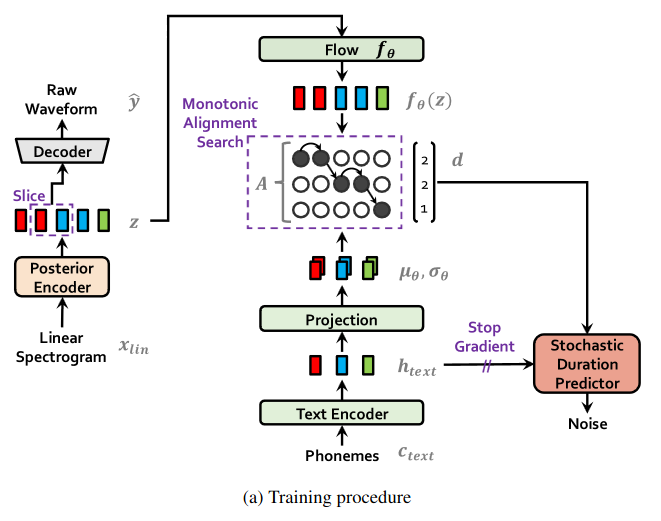
\includegraphics[scale=0.4]{imgs/vits/training.png}
    \caption{VITS training procedure}
    \label{fig:vits-training}
\end{figure}
\begin{figure}[htb]
    \centering
    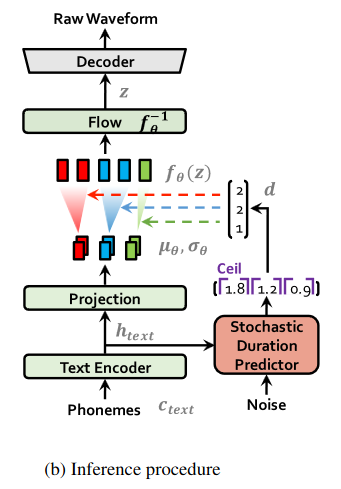
\includegraphics[scale=0.4]{imgs/vits/inference.png}
    \caption{VITS inference procedure}
    \label{fig:vits-inference}
\end{figure}

The VAE part of the is the left part of the model in fig.~\ref{fig:vits-training} where there is a Posterior Encoder that takes
a spectrogram ($x_{lin}$) of the training audio and transforms it to a lower dimensional latent space and 
a decoder to take the latent vector ($z$) and try and retrieve the original waveform.

The right side of the model in fig.~\ref{fig:vits-training} is the part that is trying to estimate an alignment between 
the speech and the input text using Monotonic Alignment Search (MAS). MAS was introduced in Glow-TTS \cite{glowtts}
and tries to maximize the likelihood of the input speech latent.
The model also has prior distributions on several components (green blocks in Fig.~\ref{fig:vits-training})
that are changed as more data is input into the model. The flow model is used here to allow a
invertible transformation of a simple distribution to a complex distribution. The invertible part is important
for the model at inference.
In addition, the durations of the speech vectors 
are passed to a Stochastic Duration Predictor for the realistic rhythms mentioned before.
Lastly, the entire model is trained with an adversarial network (not shown in Fig.~\ref{fig:vits-training})
that tries to discriminate the output of the decoder.

The inference model in fig.~\ref{fig:vits-inference} has a few changes to the training model:
\begin{enumerate}
    \item The encoder is discarded because speech is not an input to the inference model.
    \item The alignment is now used to predict a function of the latent vector from input text and the durations
    generated by the Stochastic Duration Predictor.
    \item The Normalizing Flow model is inverted to obtain the latent vector that is then passed to the decoder
    for the final waveform.
\end{enumerate}

\subsubsection{So-VITS-SVC}
SoftVC VITS Singing Voice Conversion aims to clone another persons voice on top of an input of a source audio.
It aims to keep the tones and intonation while still making the voice sound as close to the cloned voice as possible.
This project does not have a paper associated with it and thus we are unsure of what exactly their
architecture they have for their training and inference process. However, we can make some educated
guesses on what is actually happening by looking that tools they used and their statement on the model:
"The singing voice conversion model uses SoftVC content encoder to extract speech features from the source audio. These feature vectors are directly fed into VITS without the need for conversion to a text-based intermediate representation. As a result, the pitch and intonations of the original audio are preserved. Meanwhile, the vocoder was replaced with NSF HiFiGAN to solve the problem of sound interruption." \cite{sovitssvc-repo}

They used SoftVC \cite{softvc} to extract these "feature vectors" from the source audio which aims to use
distributions of these "features" instead of discrete features. Using these soft features, the output audio becomes 
more natural compared to using the discrete features.

In the repo, they stated that these features are then fed directly into a VITS model, avoiding the Text Encoder
part of the model and preserves the original intonations of the audio (Fig.~\ref{fig:vits-training}).

Another change would is to the "vocoder" which in this repo describes the "decoder" in the VITS model (Fig.~\ref{fig:vits-training})

\subsubsection{TorToiSeTTS}

TorToiSeTTS \cite{ttts} is composed of the following parts: first, an autoregressive decoder which predicts a probability distribution of speech tokens. Then a contrastive model, CVLP, is used to rank the outputs from the autoregressive decoder, producing a correlation score for each speech candidate and the text. The top k speech candidates are then chosed and a denoising diffusion probability model (DDPM) is used to convert this into a MEL speech spectrogram. Reptition penalty and temperature can be configured during the diffusion process to obtain variations in the output waveform.

\begin{figure}[htb]
    \centering
    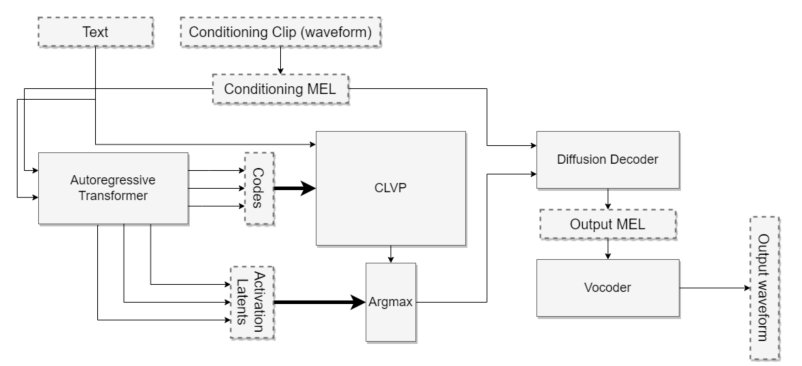
\includegraphics[scale=0.65]{tortoisefigure2.png}
    \caption{The Tortoise TTS design diagram, showing how input text is transformed into an output waveform.}
    \label{fig:tortoise}
\end{figure}

We used a significantly optimized version of Tortoise by using api\_fast.py \cite{fasttortoise} that performs around 5 to 10 times faster than the original version. This is due to a number of optimizations, including using KV cache to speed up sampling, using half precision whenever possible, and a better diffusion sampling method (dpm++2m).

\subsection{LLM}
OpenAI does not publish the technical details of their recent GPT models (GPT-3.5 and GPT-4) however, we can draw
parallels to the GPT-2 \cite{gpt2} models that they have published the technical details on.
The GPT \cite{gpt} architecture uses a Transformer based architecture that takes in tokens and tries to
predict the tokens that should follow the input.

\subsection{Stable Video Diffusion}

The architecture is similar to an image diffusion model, and a pretrained image diffusion model can be used to create the video diffusion model. Stable Video Diffusion \cite{svd} says that they use the same architecture from an earlier model \cite{align}. This earlier model uses a combination of spacial and temporal convolution and attention layers where there is a temporal layer is inserted between the spacial layers that existed in the original image diffusion model and can be seen in Fig.~\ref{fig:temporal}.

\begin{figure}[htb]
    \centering
    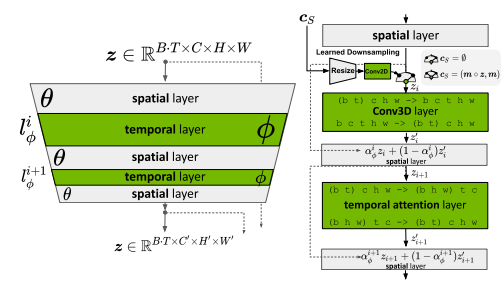
\includegraphics[scale = 0.9]{svd img 1.png}
    \caption{Temporal and Spatial Layers in SVD Model}
    \label{fig:temporal}
\end{figure}

The network is then trained by freezing the spacial layers and only optimizing the temporal layers. Additional fine tuning with video data is performed on all layers to remove artifacts, such as flickering. Note that while video content used for initial training is at a low resolution, high resolution video is used for this fine tuning stage. \\


 The WebVid-10M dataset is used for training. A curation process to filter out only desirable videos from all of the data was a crucial step for generating high quality results. IN particular, any video containing jump cuts is detected and either used as separate video sequences or not used. 
 
 The video generation process takes in a CLIP image embedding of the input image, and first generates sparse keyframes with large semantic changes in latent space, performs interpolation between those keyframes, then decodes it into pixel space. Although there is no strict limit to how long the video generated can be, available memory poses a barrier to longer videos, and the attention network only attends to at most the last 8 frames. SVD currently comes in a 14 frame and 25 frame version, with us using the 25 frame version. 
 
 Additionally, the guidance scale for image to video is increased linearly over the duration of each video clip generation, as the researchers have found that this leads to fewer artifacts and inconsistencies. Camera tracking LoRAs were also trained, specifically on horizontal panning, zooming and static perspectives.

\begin{figure*}[ht]
    \centering
    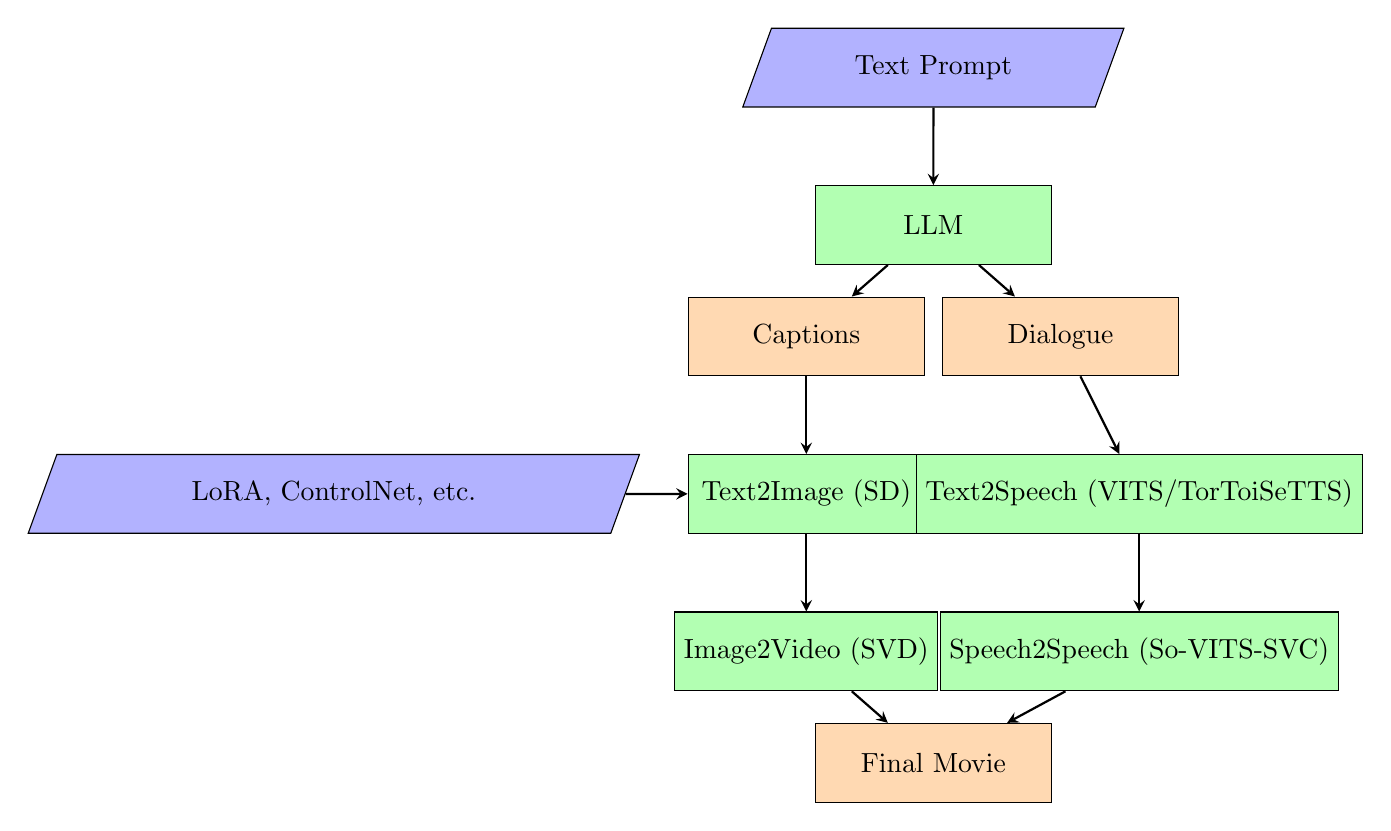
\begin{tikzpicture}[node distance=2cm]
    \node (in) [io] {Text Prompt};
    \node (LLM) [process, below of=in, fill=green!30] {LLM};
    \node (Captions) [process, below left of=LLM, xshift=-0.2cm] {Captions};
    \node (Dialogue) [process, below right of=LLM, xshift=0.2cm] {Dialogue};
    \node (Text2Image) [process, below of=Captions, fill=green!30] {Text2Image (SD)};
    \node (SDOptions) [io, left of=Text2Image, xshift=-4.0cm] {LoRA, ControlNet, etc.};
    \node (Text2Speech) [process, below of=Dialogue, fill=green!30, xshift=1.0cm] {Text2Speech (VITS/TorToiSeTTS)};
    \node (Image2Video) [process, below of=Text2Image, fill=green!30, xshift=-0.0cm] {Image2Video (SVD)};
    \node (Speech2Speech) [process, below of=Text2Speech, fill=green!30, xshift=0.0cm] {Speech2Speech (So-VITS-SVC)};
    \node (Final Movie) [process, below left of=Speech2Speech, xshift=-1.2cm] {Final Movie};
    \draw [arrow] (in) -- (LLM);
    \draw [arrow] (LLM) -- (Captions);
    \draw [arrow] (LLM) -- (Dialogue);
    \draw [arrow] (Captions) -- (Text2Image);
    \draw [arrow] (Dialogue) -- (Text2Speech);
    \draw [arrow] (Text2Image) -- (Image2Video);
    \draw [arrow] (SDOptions) -- (Text2Image);
    \draw [arrow] (Text2Speech) -- (Speech2Speech);
    \draw [arrow] (Image2Video) -- (Final Movie);
    \draw [arrow] (Speech2Speech) -- (Final Movie);
    \end{tikzpicture}
    \caption{Flowchart of Pipeline}
    \label{fig:pipeline}
\end{figure*}

\begin{figure*}[ht]
    \begin{center}
        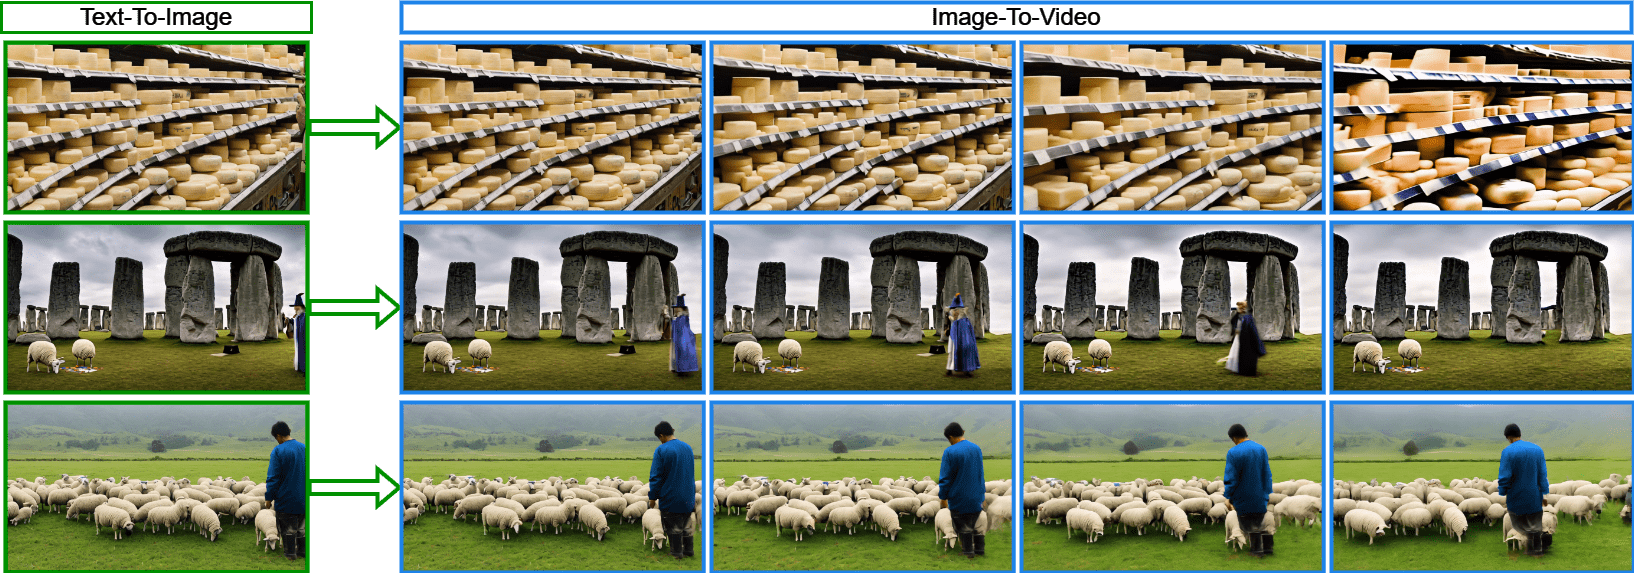
\includegraphics[width=0.8\textwidth]{imgs/final-intermediate/sd_to_svd.png}
    \end{center}
    \caption{Examples for Text-To-Video synthesis}
    \label{fig:ttv}
\end{figure*}

\begin{figure*}[ht]
    \begin{center}
        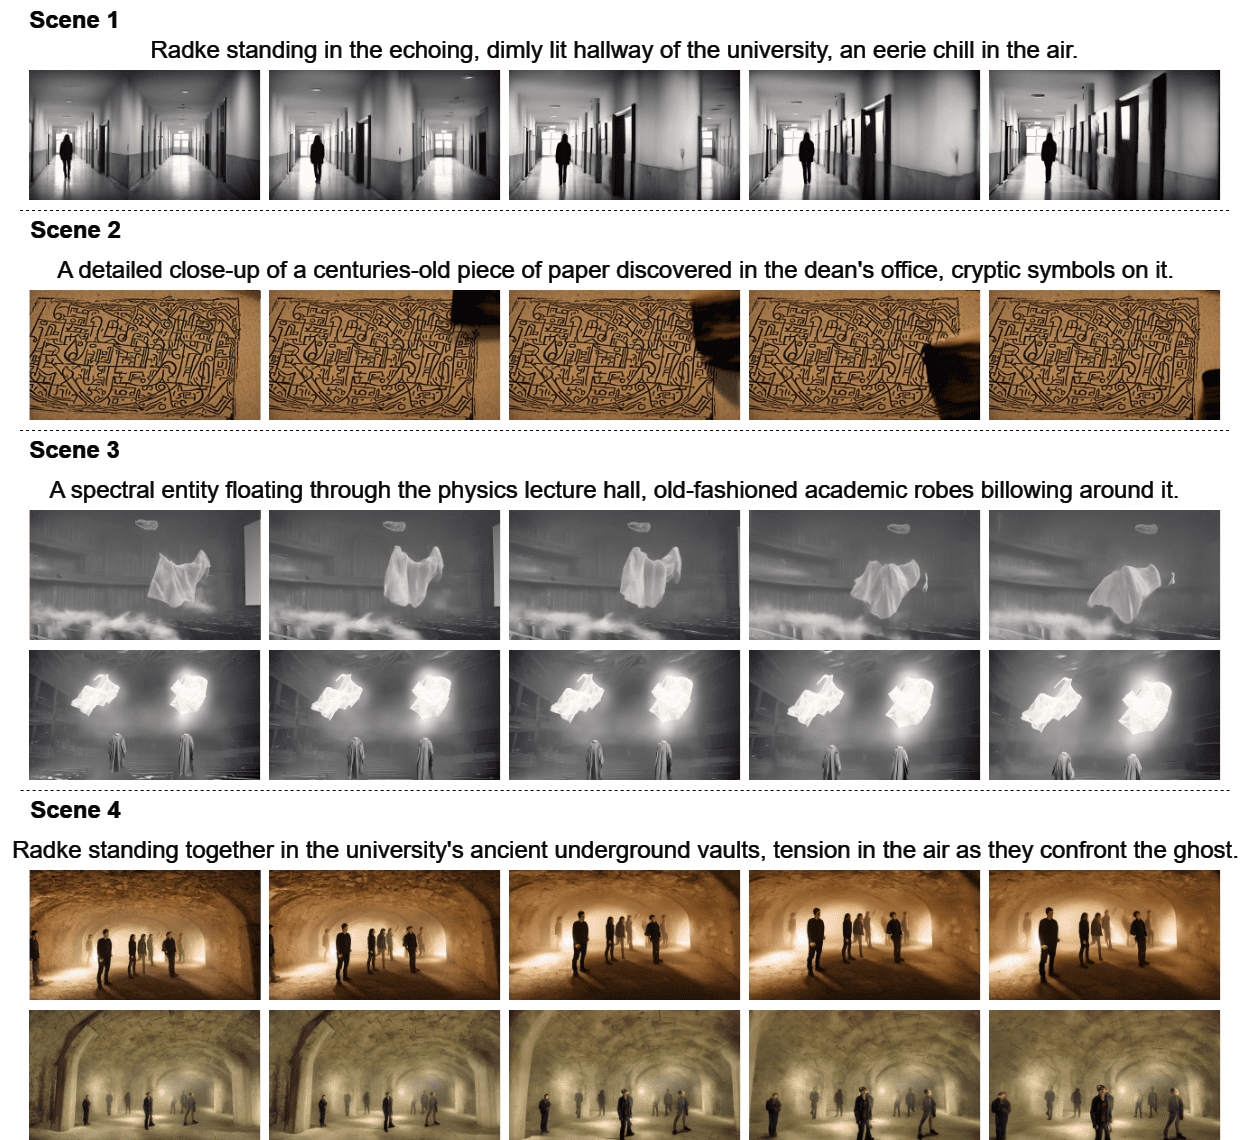
\includegraphics[width=0.8\textwidth]{imgs/final-intermediate/scenes.png}
    \end{center}
    \caption{Result for an entire script of scenes including the captions}
    \label{fig:script}
\end{figure*}


\subsection{Pipeline}
Our pipeline for generating the scenes includes several different projects: an LLM \cite{gpt4}, 
SD \cite{stablediffusion}, SVD \cite{svd}, VITS \cite{vits}/TorToiSeTTS\cite{ttts}, and So-VITS-SVC \cite{sovitssvc-repo}.

\begin{enumerate}
    \item User creates a text prompt describing for a scene or event.
    \item The LLM generates the dialogue and caption describing each scene.
    \item Each caption is passed to SD to a image of what the caption is describing.
    \item Each image is passed to SVD to get a video clip of what the caption is describing.
    \item Each dialogue is passed to VITS or TorToiSeTTS to generate a voice-over.
    \item (OPTIONAL) Each voice-over is passed to So-VITS-SVC to apply a cloned voice onto the voice-over.
    \item Each video and voice-over is combined to make a final movie.
\end{enumerate}
For clarification, refer to the flowchart of our pipeline: ''Fig.~\ref{fig:pipeline}''.

\section{Intermediate Results}

\begin{tcolorbox}
Include some “making of” information and images that illustrate steps in
creating the various elements of your project. That is, don’t just show the final result, show some of the underlying pieces you needed to create the effect (e.g., guidance images for ControlNet, input images for textual inversion, prompts for Stable Diffusion, etc.). Highlight both strengths of your current algorithms and weaknesses that you didn’t have time to fix or had to find a quick solution to. I would like to see lots of images and discussion here!
\end{tcolorbox}

\subsection{LLM}

Our intermediate steps are according to our flowchart of the pipeline: Figure 3. First, we take a user input as a text prompt, this prompt is sent to a LLM that generates a story based on that prompt. The LLM receives an example of the prompt, and we prompt engineer the LLM to create a response that would follow our format for the generation of a movie. The example we use is as described:

\begin{verbatim}
{
"characters": [
    {"name": "Radke"}
],
"style": "realistic",
"script": [ 
    {"caption": "A sheep looking at cheese 
    in a supermarket.", 
    "dialogue": [
        {"character": "Radke", "text": "In 
        the mist-enshrouded hills of an 
        ancient land, there lies a 
        mystery as old as time itself. 
        Behold the enigmatic sheep, 
        creatures shrouded in the lore 
        and legend of yesteryears."}
    ]
    }
]
}
\end{verbatim}

Then we send the system as a role where they are a TV show writer, and that they have to generate the "prompt" by filling in a .json file, the style described in the example. In our earlier cases, we generated scripts that were too long, it had around 20 captions and 5 dialogue pieces per caption. This took up too much memory, and due to a limited amount of time for testing, we engineered the prompt to keep the script around with 4 captions and a maximum of 2 characters per caption speaking. This prevented us from running out of memory and produced quick movies as results. 

Once the LLM has produced a script for us to use, we take the script and derive it into a list of generations. This contains the character, their dialogue, and their caption. Each item in the list will be sent to various algorithms for their generation. From now, when we iterate through the list, it will take the $i^{th}$ iteration and generate according to that iteration. For instance, if we have captions that are 3 long, and for each caption we have a 2 dialogues. In the 3rd list sequence, it is the 1st dialogue of the 2nd caption, in which includes a character speaking that dialogue. Here is a visual example:

\begin{verbatim}
1st: [character: John, caption: "There is 
a ghost in the hallway", dialogue: 
"I am scared of phantoms"]
2nd: [character: Ghost, caption: "There 
is a ghost in the hallway", 
dialogue: "Boo!"]
3rd: [character: John, caption: "A 
ghost appears next to John", 
dialogue: "Ahhhh!"]
\end{verbatim}

Although we generated impressive results with no issues on the end of LLM, we are using credits through OpenAI's GPT-4. This is a paid service and thus not possible to be provided in a large capacity. We have tried other LLMs, including Meta's Llama 2 \cite{llama2}, it did not work as well as GPT-4 in generating a cohesive example according to the layout. Therefore, we left it out as a future budget option that we can incorporate.

\subsection{Text2Speech}

First, we have the audio generation, this takes in the dialogue at the $i^{th}$ iteration in the list. Next, this dialogue is sent to a text-to-speech (tts) module, that would generate a voice sample. According to different implementations of our current pipeline, these results would go two ways. Both include various steps and have their own respective advantage. Most of our results use TorToiSeTTS, if you hear that a result includes Prof. Radke's voice, it is utilizing So-VITS-SVC. \\

Before any inferencing, we have an initial step before generating any TTS samples. This step is to take the list of characters in the dialogue, and assign various voice actors to the specific character.

\subsubsection{TorToiSeTTS}

This model currently supports than 7 characters, and will repeat assignment if exceeding 7 (if the prompt determines so). Once the dialogue with that specific character is chosen, the TTS is enabled with inference on. The dialogue at the $i^{th}$ iteration in the list is then sent into the model for inference and results in an audio file. The API we use for TorToiSeTTS is without diffusion, this makes the inference much faster. This API is developed in the fast\_api code in the author's repository. 

\begin{center}
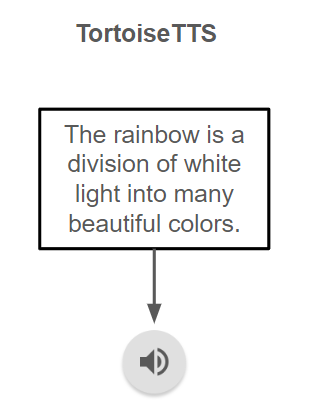
\includegraphics[width=0.2\textwidth]{imgs/final-intermediate/ttts.png}\\
\end{center}

This is saved in an audio file and accessed later in order to clear the cache and save memory for following models.

\subsubsection{VITS}
If we are not using TorToiSeTTS for our TTS samples, VITS is used instead. The only models available to us are the pretrained models used in their demo \cite{vits-demo}. A similar selection of characters will happen with the available VITS models that in present in the models folder. The dialogue at the $i^{th}$ iteration in the list is then sent into the model for inference and results in an audio file. Similar to the tortoise implementation.

\begin{center}
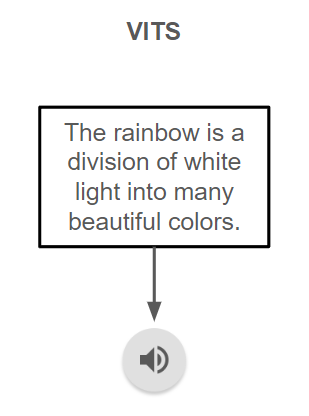
\includegraphics[width=0.2\textwidth]{imgs/final-intermediate/vits.PNG}\\
\end{center}

\subsubsection{So-VITS-SVC}
If the user wants to have one of the characters to be one of the voices that are cloned, then the
audio files generated by VITS is passed into the So-VITS-SVC module and a audio file with the
cloned voice is generated and saved.
The only model that we have trained currently is the one of Professor Radke, and we found that
the male VITS model with So-VITS-SVC performs better than using TorToiSeTTS with So-VITS-SVC.

\begin{center}
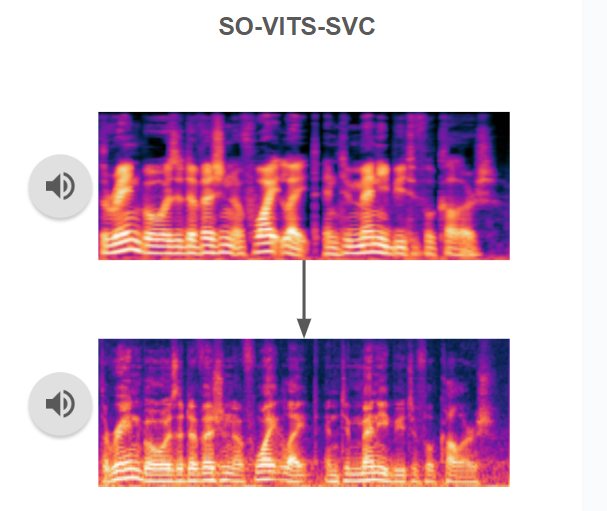
\includegraphics[width=0.2\textwidth]{imgs/final-intermediate/sovits.PNG}\\
\end{center}

\subsection{Text2Video}

Next, we have the video generation, this takes the captions at the $i^{th}$ iteration in the list. Next, this caption is sent to a text-to-image synthesizer, which will generate an image based on the content of the captions. The text is sent to a text-to-image synthesizer, in this case we use Stable Diffusion \cite{stablediffusion}. Here, the caption is sent to generate an image:

\begin{center}
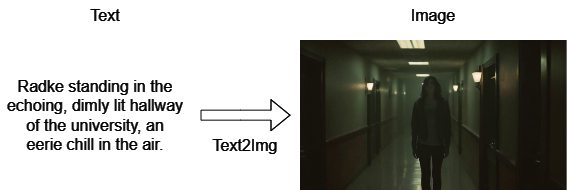
\includegraphics[width=0.4\textwidth]{imgs/final-intermediate/t2i_intermediate.png}\\
\end{center}

Then, we take that single image, and send it to an image-to-video synthesizer, in this case we use Stable Diffusion Video \cite{svd} (SVD) to create multiple frames of images from the original image generated by the text-to-image model. With the previous model, we create a text-to-video framework. We include multiple examples of this in ''Fig.~\ref{fig:ttv}''.

Since SVD can only generate a maximum of 25 frames, we presume that the audio given at a particular dialogue will most likely not reach 25 frames. Therefore, we created a loop that would take the last frame of the generation, which is an image. Then we would send that to SVD to create a video again. This step continues until the audio ends, and the amount of frames it takes for the audio to end is calculated through the sampling ratio of our audio sample. This step has led to some good results, but had some weird results as well. We will explain in more detail in our final frames.

\subsection{Scene: Synthesis of Video \& Audio}

Finally, all of the frames and audio are combined to create a scene. After all of the scenes are created, the music, if needed, is added to the end. The output includes all of the scenes rendered as a .mp4 file. ''Fig.~\ref{fig:script}'' includes an example of the result including the captions.

\section{Final Frames}
\begin{tcolorbox}
Show some sequences of final outputs/images where you feel that the algorithms worked particularly well. Also, show some outputs/images that didn’t work so well and critically assess what happened.
\end{tcolorbox}

\subsection{\textbf{Prompt}: make a commercial where Dwayne "the rock" Johnson sells orange juice}

\begin{center}
\includegraphics[width=0.4\textwidth]{imgs/final-intermediate/rock.png}
\end{center}

In our current example we have the first SVD generation of the rock moving forward in the grocery store. However, in the second generation by taking the frame of the last frame of the initial frames, he started to walk backwards. This is due to the fact that between those generations, we do not keep any spatial or temporal consistency, and thus, the rock, randomly decided to walk backwards. On the other hand, there are instances where this works well.

\begin{center}
\includegraphics[width=0.4\textwidth]{imgs/final-intermediate/rock2.png}
\end{center}

We presume that it is able to keep the walking animation because it is easier to keep a temporal consistency when the next action is easily predictable: walking forward. Whereas, in our first example, it is hard to tell if the rock is moving forward or backward by just looking at one image. We perceive that a person is walking forward in that instance.

\subsection{\textbf{Prompt}: gordon ramsay going to the hospital after eating too many burgers}

\begin{center}
\includegraphics[width=0.4\textwidth]{imgs/final-intermediate/gordon.png}
\end{center}

If we look at the individual frames, many images kept spatial and temporal consistency. It appears that Gordon Ramsay eats a burger, but it cannot animate the act of eating that burger. In the final scene, it was able to correctly animate his hand moving. These examples did not include any additional frames, and held temporal consistency almost throughout. Therefore, it held good results for most of the generation.

Additionally, a prevalent issue arises because we do not have the genders of the characters in the script so a female voice actor can be selected when generating the speech for a male character. In this example,
a female voice actor was chosen for Gordon Ramsey
This video and other examples can be found in the class Box or the Github repo since we
are unable to play videos in PDF files.

\subsection{\textbf{Prompt}: Italian mobsters start an advertisement for a pizza company}

\begin{center}
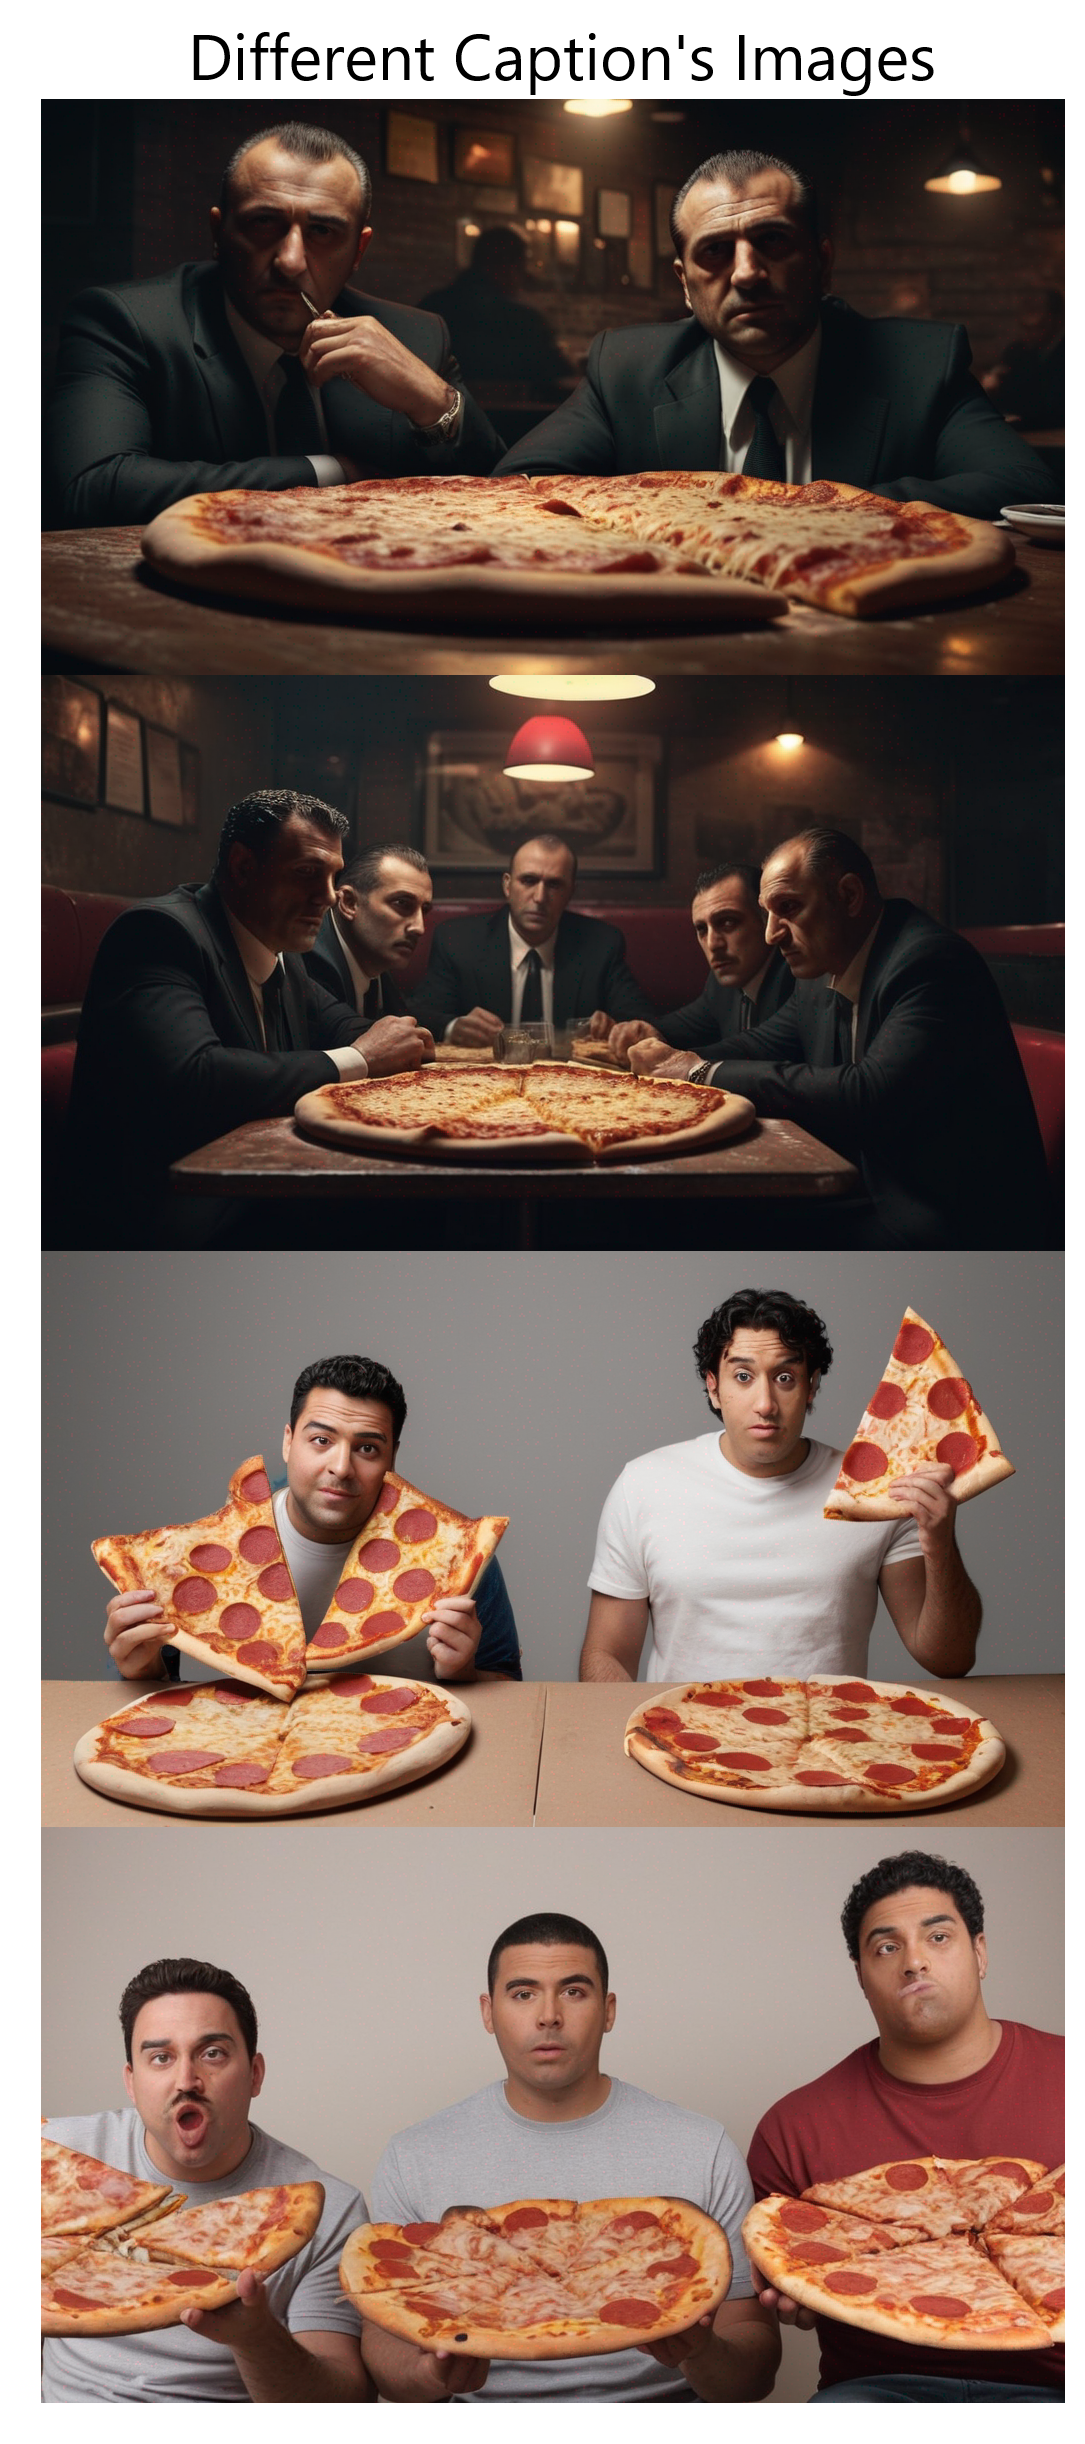
\includegraphics[width=0.25\textwidth]{imgs/final-intermediate/pizza.png}
\end{center}

In this example, we can see that Stable Diffusion was able to generate 
stereotypical mobsters for the first two scenes but once the captions
stopped mentioning that the characters were mobsters, normal
looking characters were generated instead. This issue of
character (temporal) consistency between difference scenes
can be somewhat fixed by making sure that the captions always have
the relevant context for the prompt.

% \subsection{Results}
% We have created an example where the text prompt is "Walter White baking" (\href{https://www.youtube.com/watch?v=lsVTRfqRHe0}{Youtube Link}).
% The clips were generated by a non-fine-tuned Text2Video-Zero \cite{text2vid} and a pre-trained model
% on Walter White's voice actor on FakeYou (\href{https://fakeyou.com/about}{Link}). FakeYou was
% only used to create the voice-over for this example, we plan on using open-source models like
% VITS \cite{vits} for the final project. The
% video clips and voice-overs were stitched together manually to 
% create a prototype of what a final movie would look like.

% Here is an example of the script that GPT-4 \cite{gpt4} generated in response to our prompt:
% \begin{tcolorbox}
% \begin{lstlisting}
%     {
%       "characters": [
%         {"name": "Walter White"}
%       ],
%       "mood": "",
%       "background-sound": 
%         {"link":"path/to/music"},
%       "script": [ 
%         {"caption": "Walter White baking bread", "dialogue": [
%           {"character": "Walter White", "text": "My name is Walter Hartwell White..."}
%         ] }
%       ]
%     }
% \end{lstlisting}
% \end{tcolorbox}
% \subsection{Reflection}
% Here are some potential issues with text-to-video synthesis that we came across when generating the result and here are our potential fixes and fixes that we had:
% (* denotes that it is our current solution to the problem)
% \begin{itemize}
%     \item text-to-video synthesis only created suitable results at a general 40-50 inferences with a capped frame count of 24. If we tried to generate more frames it would not effectively create a video (we tried 48 frames and it generated something random, that is because the model was trained to run with 24 frames). 
%     \begin{itemize}
%         \item we can try to extend the video by taking a frame and translating that to another video
%         \item * we can just create multiple 3 second videos with the same caption if we need to extend the single clip
%     \end{itemize}
%     \item text-to-video synthesis can sometimes generate a setting that can be vastly different from each other. If you look at Figure ~\ref{fig:mood}, you can see that there are two videos, both of which are generated. One of them has a brighter setting and the other a dim and darker one. Thus, our problem is consistency.
%     \begin{itemize}
%         \item * Not completely sure, since if we have a less generalized prompt, it may be worse for the end product, but a potential solution is to add the mood to the end of the caption. So if we had "walter white baking bread" and the mood as "a bright sunny day", we can add the caption and the mood as an input. (i.e. walter white baking bread during a bright sunny day").
%     \end{itemize}
% \end{itemize}

% \begin{figure}[h]
%     \centering
%     \begin{subfigure}[b]{0.5\textwidth}
%         \centering
%         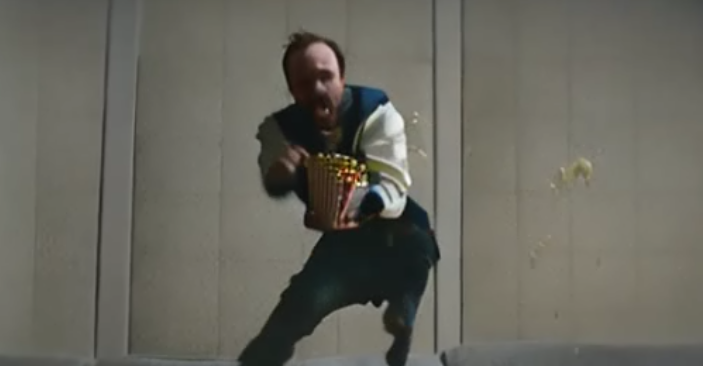
\includegraphics[width=\textwidth]{light.png}
%         \caption{Jesse Pinkman throws his popcorn bowl on the floor and jumps out of his sofa with excitement}
%     \end{subfigure}
%     \begin{subfigure}[b]{0.5\textwidth}
%         \centering
%         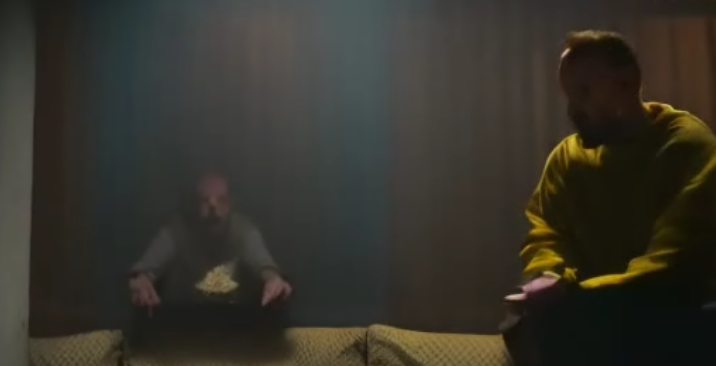
\includegraphics[width=\textwidth]{dark.png}\caption{Walter White and Jesse Pinkman sitting at a sofa both reaching for the popcorn bowl}
%     \end{subfigure}
%     \caption{Various moods without clarification}
%     \label{fig:mood}
% \end{figure}


\section{Discussion and Further Work}

\begin{tcolorbox}
If you had more time to work on this project, what else could you do
to make it better? Now that you completed the project, what would you have done differently (e.g., in terms of the original data you collected or networks you tried)? What are some extensions based on concepts from the course that could apply to your project?
\end{tcolorbox}

\subsection{Further Work}
In our project, the method to generate a movie form a text is an end to end process that is completely automated. However, we added a manual script to include music in the video, this required the user to add the music file in the repository or use the one we already have. Then, they would have to add this as a command to include in the final video. We have not experimented much with this idea, but I think it would add an extension to the project that would be interesting. 

Another idea that we have no delved too deep in, is fine-tuning a model that would generate in a particular style or stay consistent with the previously generated style. For instance, we found that one model really liked to generate cartoons, and then add one realistic image. In order to alleviate this, we added a custom parameter that included the style to stable diffusion. This is a novel approach since many images generated with a particular style maintain that style. However, as we tried this method with "realism" as a style tag, it still generated cartoon images through stable diffusion. Therefore, this was an imperative issue that we would investigate more into, if we had more time for the project. 

Additionally, to that similar issue, we had experimented with many different stable diffusion versions, styles, and even the newest stable diffusion release for our text-to-image synthesis. Before concluding that the newest, fine-tuned Stable Diffusion XL, had the best results out of all the other models. This could have definitely saved us more time in inferencing results, since we had tested many different results over time and different model versions. \\

As we described under intermediate frames, we would like to experiment more with SVD generating more temporal and spatial frames in the future generations. However, this would involve delving into the model in order to keep future images with that same consistency. Therefore, we kept our current solution as of now, and may look into this as further work. \\

Finally, we need more time to experiment with So-VITS-SVC to work with the TorToiSeTTS model. In our initial result, when we used speech-to-speech, it dampened the voice and sometimes it even cuts out the audio after inference. This is an error that our group has not figured out yet after various trials and tests. We believe that it might be due to the hyperparameters that it uses, since it is defaulted to VITS. Perhaps it might be better to find the optimal hyperparameters for TorToiSeTTS.

\subsection{Extensions}

% add AI music
We mentioned previously that we would experiment and attempt to extent AI generated music to add as a mood to the scene. This would completely make our results automated, including music. In class, we mentioned various music generators, for instance, a GAN-inspired music generator: GANSynth \cite{GANSynth}. This would be an improve to our current pipeline and could be an effective extension mentioned in class. Yet, this does introduce more problems that we would have to assume that the LLM can generate. For instance, we know that a comedic sketch will include lighthearted jingles, but that mood is not always consistent with what music it needs to be generated. If we are using a particular LLM to predict what it should generate, it is another layer of abstraction that could lead to issues in the future. Whereas, by manually selecting the music, we are able to derive what the mood or tone should be. \\

Moreover, in our original concept, we just applied stable diffusion for a simple image. We can include multi-model support and support for plugins for other models like DreamBooth \cite{dreambooth} or ControlNet \cite{controlnet}. In our personal homeworks, we have utilized ControlNet and LoRA \cite{lora} with Stable Diffusion in order to generate a particular character in the scene doing various tasks. We can possibly apply that to our project, and create a more descriptive storytelling method by having that particular character on those scenes. Furthermore, Algoleafic Art, created a storytelling module that created specific images of characters that are temporally consistent between scenes. Therefore, we can apply that logic and try to keep our scenes consistent between one character. 

\begin{thebibliography}{00}

\bibitem{text2vid} L. Khachatryan et al., Text2Video-Zero: Text-to-Image Diffusion Models are Zero-Shot Video Generators. 2023. \href{https://arxiv.org/pdf/2303.13439.pdf}{Reference Link}

\bibitem{text2vid-gh} Picsart-AI-Research (2023) Text2Video-Zero [Source Code]. \href{https://github.com/Picsart-AI-Research/Text2Video-Zero}{Github Link}

\bibitem{stablediffusion} R. Rombach et al., High-Resolution Image Synthesis with Latent Diffusion Models. 2022. \href{https://arxiv.org/pdf/2112.10752.pdf}{Reference Link}

\bibitem{dreambooth} N. Ruiz et al., DreamBooth: Fine Tuning Text-to-Image Diffusion Models for Subject-Driven Generation. 2023. \href{https://arxiv.org/pdf/2208.12242.pdf}{Reference Link}

\bibitem{controlnet} Zhang, Lvmin, et al., Adding Conditional Control to Text-to-Image Diffusion Models. 2023. \href{http://arxiv.org/abs/2302.05543.}{Reference Link}

\bibitem{gpt4} OpenAI, GPT-4 Technical Report. 2023. \href{https://arxiv.org/pdf/2303.08774.pdf}{Reference Link}

\bibitem{gpt2} A. Radford et al., Language Models are Unsupervised Multitask Learners. 2019. \href{https://d4mucfpksywv.cloudfront.net/better-language-models/language_models_are_unsupervised_multitask_learners.pdf}{Reference Link}

\bibitem{gpt} A. Radford et al., Improving Language Understanding by Generative Pre-Training. 2018. \href{https://s3-us-west-2.amazonaws.com/openai-assets/research-covers/language-unsupervised/language_understanding_paper.pdf}{Reference Link}

\bibitem{llama} H. Touvron, T. Scialom et al., Llama 2: Open Foundation and Fine-Tuned Chat Models. 2023. \href{https://arxiv.org/pdf/2307.09288.pdf}{Reference Link}

\bibitem{vits} J. Kim, J. Kong, and J. Son, Conditional Variational Autoencoder with Adversarial Learning for End-to-End Text-to-Speech. 2021.\href{https://arxiv.org/pdf/2106.06103.pdf}{Reference Link}

\bibitem{vits-demo} jaywalnut310 (2021) VITS-Demo [Source Code]. \href{https://jaywalnut310.github.io/vits-demo/index.html}{Github Link}

\bibitem{glowtts}  Jaehyeon Kim et al., Glow-TTS: A Generative Flow for Text-to-Speech via Monotonic Alignment Search. 2020. \href{https://arxiv.org/pdf/2005.11129.pdf}{Reference Link}

\bibitem{sovitssvc-repo} svc-develop-team (2023) So-VITS-SVC Repo [Source Code]. \href{https://github.com/svc-develop-team/so-vits-svc}{Github Link}

\bibitem{softvc} Benjamin van Niekerk et al., A Comparison of Discrete and Soft Speech Units for Improved Voice Conversion. 2021 \href{https://arxiv.org/abs/2111.02392}{Reference Link}

\bibitem{svd} A. Blattmann et al., Stable Video Diffusion: Scaling Latent Video Diffusion Models to Large Datasets. 2023. \href{https://arxiv.org/abs/2311.15127}{Reference Link}

\bibitem{align} Andreas Blattmann et al., Align your Latents: High-Resolution Video Synthesis with Latent Diffusion Models. 2023. \href{https://arxiv.org/pdf/2304.08818.pdf}{Reference Link}

\bibitem{lora} Edward J. Hu et al., LoRA: Low-Rank Adaptation of Large Language Models. 2021. \href{https://arxiv.org/pdf/2106.09685.pdf}{Reference Link}

\bibitem{GANSynth} Engel, J., Agrawal, K. K., Chen, S., Gulrajani, I., Donahue, C., \& Roberts, A. GANSynth: Adversarial Neural Audio Synthesis. International Conference on Learning Representations. 2019. \href{https://openreview.net/forum?id=H1xQVn09FX}{Reference Link}

\bibitem{llama2} Touvron, H., Martin, L., Stone, K., Albert, P., Almahairi, A., Babaei, Y., ... Scialom, T. Llama 2: Open Foundation and Fine-Tuned Chat Models. 2023. \href{http://arxiv.org/abs/2307.09288}{Reference Link}

\bibitem{breakingbread} [Kneeco]. I asked ai to make a Walter White bakery commercial. 2023. \href{https://www.youtube.com/watch?v=dgkZTHHom94}{Reference Link}

\bibitem{minecraft} [Presidents Play]. US Presidents Play Minecraft. 2023. \href{https://www.youtube.com/watch?v=qYF0jhwrzxA}{Reference Link}

\bibitem{ttts} Betker, James. Better speech synthesis through scaling. 2023. \href{https://arxiv.org/pdf/2305.07243.pdf}{Reference Link}

\bibitem{fasttortoise} Betker, J. (2022). TorToiSe text-to-speech. \href{https://github.com/neonbjb/tortoise-tts/blob/main/tortoise/api_fast.py}{GitHub Link}

\end{thebibliography}

\end{document}
